% Generated by Sphinx.
\def\sphinxdocclass{report}
\documentclass[letterpaper,10pt,polish]{sphinxmanual}
\usepackage[utf8]{inputenc}
\DeclareUnicodeCharacter{00A0}{\nobreakspace}
\usepackage[T1]{fontenc}
\usepackage{babel}
\usepackage{times}
\usepackage[Sonny]{fncychap}
\usepackage{longtable}
\usepackage{sphinx}


\title{Podręcznik użytkownika serwera knut Dokumentacja}
\date{2010-09-20}
\release{0.1}
\author{Wiktor Idzikowski}
\newcommand{\sphinxlogo}{}
\renewcommand{\releasename}{Wydanie}
\makeindex

\makeatletter
\def\PYG@reset{\let\PYG@it=\relax \let\PYG@bf=\relax%
    \let\PYG@ul=\relax \let\PYG@tc=\relax%
    \let\PYG@bc=\relax \let\PYG@ff=\relax}
\def\PYG@tok#1{\csname PYG@tok@#1\endcsname}
\def\PYG@toks#1+{\ifx\relax#1\empty\else%
    \PYG@tok{#1}\expandafter\PYG@toks\fi}
\def\PYG@do#1{\PYG@bc{\PYG@tc{\PYG@ul{%
    \PYG@it{\PYG@bf{\PYG@ff{#1}}}}}}}
\def\PYG#1#2{\PYG@reset\PYG@toks#1+\relax+\PYG@do{#2}}

\def\PYG@tok@gd{\def\PYG@tc##1{\textcolor[rgb]{0.63,0.00,0.00}{##1}}}
\def\PYG@tok@gu{\let\PYG@bf=\textbf\def\PYG@tc##1{\textcolor[rgb]{0.50,0.00,0.50}{##1}}}
\def\PYG@tok@gt{\def\PYG@tc##1{\textcolor[rgb]{0.00,0.25,0.82}{##1}}}
\def\PYG@tok@gs{\let\PYG@bf=\textbf}
\def\PYG@tok@gr{\def\PYG@tc##1{\textcolor[rgb]{1.00,0.00,0.00}{##1}}}
\def\PYG@tok@cm{\let\PYG@it=\textit\def\PYG@tc##1{\textcolor[rgb]{0.25,0.50,0.56}{##1}}}
\def\PYG@tok@vg{\def\PYG@tc##1{\textcolor[rgb]{0.73,0.38,0.84}{##1}}}
\def\PYG@tok@m{\def\PYG@tc##1{\textcolor[rgb]{0.13,0.50,0.31}{##1}}}
\def\PYG@tok@mh{\def\PYG@tc##1{\textcolor[rgb]{0.13,0.50,0.31}{##1}}}
\def\PYG@tok@cs{\def\PYG@tc##1{\textcolor[rgb]{0.25,0.50,0.56}{##1}}\def\PYG@bc##1{\colorbox[rgb]{1.00,0.94,0.94}{##1}}}
\def\PYG@tok@ge{\let\PYG@it=\textit}
\def\PYG@tok@vc{\def\PYG@tc##1{\textcolor[rgb]{0.73,0.38,0.84}{##1}}}
\def\PYG@tok@il{\def\PYG@tc##1{\textcolor[rgb]{0.13,0.50,0.31}{##1}}}
\def\PYG@tok@go{\def\PYG@tc##1{\textcolor[rgb]{0.19,0.19,0.19}{##1}}}
\def\PYG@tok@cp{\def\PYG@tc##1{\textcolor[rgb]{0.00,0.44,0.13}{##1}}}
\def\PYG@tok@gi{\def\PYG@tc##1{\textcolor[rgb]{0.00,0.63,0.00}{##1}}}
\def\PYG@tok@gh{\let\PYG@bf=\textbf\def\PYG@tc##1{\textcolor[rgb]{0.00,0.00,0.50}{##1}}}
\def\PYG@tok@ni{\let\PYG@bf=\textbf\def\PYG@tc##1{\textcolor[rgb]{0.84,0.33,0.22}{##1}}}
\def\PYG@tok@nl{\let\PYG@bf=\textbf\def\PYG@tc##1{\textcolor[rgb]{0.00,0.13,0.44}{##1}}}
\def\PYG@tok@nn{\let\PYG@bf=\textbf\def\PYG@tc##1{\textcolor[rgb]{0.05,0.52,0.71}{##1}}}
\def\PYG@tok@no{\def\PYG@tc##1{\textcolor[rgb]{0.38,0.68,0.84}{##1}}}
\def\PYG@tok@na{\def\PYG@tc##1{\textcolor[rgb]{0.25,0.44,0.63}{##1}}}
\def\PYG@tok@nb{\def\PYG@tc##1{\textcolor[rgb]{0.00,0.44,0.13}{##1}}}
\def\PYG@tok@nc{\let\PYG@bf=\textbf\def\PYG@tc##1{\textcolor[rgb]{0.05,0.52,0.71}{##1}}}
\def\PYG@tok@nd{\let\PYG@bf=\textbf\def\PYG@tc##1{\textcolor[rgb]{0.33,0.33,0.33}{##1}}}
\def\PYG@tok@ne{\def\PYG@tc##1{\textcolor[rgb]{0.00,0.44,0.13}{##1}}}
\def\PYG@tok@nf{\def\PYG@tc##1{\textcolor[rgb]{0.02,0.16,0.49}{##1}}}
\def\PYG@tok@si{\let\PYG@it=\textit\def\PYG@tc##1{\textcolor[rgb]{0.44,0.63,0.82}{##1}}}
\def\PYG@tok@s2{\def\PYG@tc##1{\textcolor[rgb]{0.25,0.44,0.63}{##1}}}
\def\PYG@tok@vi{\def\PYG@tc##1{\textcolor[rgb]{0.73,0.38,0.84}{##1}}}
\def\PYG@tok@nt{\let\PYG@bf=\textbf\def\PYG@tc##1{\textcolor[rgb]{0.02,0.16,0.45}{##1}}}
\def\PYG@tok@nv{\def\PYG@tc##1{\textcolor[rgb]{0.73,0.38,0.84}{##1}}}
\def\PYG@tok@s1{\def\PYG@tc##1{\textcolor[rgb]{0.25,0.44,0.63}{##1}}}
\def\PYG@tok@gp{\let\PYG@bf=\textbf\def\PYG@tc##1{\textcolor[rgb]{0.78,0.36,0.04}{##1}}}
\def\PYG@tok@sh{\def\PYG@tc##1{\textcolor[rgb]{0.25,0.44,0.63}{##1}}}
\def\PYG@tok@ow{\let\PYG@bf=\textbf\def\PYG@tc##1{\textcolor[rgb]{0.00,0.44,0.13}{##1}}}
\def\PYG@tok@sx{\def\PYG@tc##1{\textcolor[rgb]{0.78,0.36,0.04}{##1}}}
\def\PYG@tok@bp{\def\PYG@tc##1{\textcolor[rgb]{0.00,0.44,0.13}{##1}}}
\def\PYG@tok@c1{\let\PYG@it=\textit\def\PYG@tc##1{\textcolor[rgb]{0.25,0.50,0.56}{##1}}}
\def\PYG@tok@kc{\let\PYG@bf=\textbf\def\PYG@tc##1{\textcolor[rgb]{0.00,0.44,0.13}{##1}}}
\def\PYG@tok@c{\let\PYG@it=\textit\def\PYG@tc##1{\textcolor[rgb]{0.25,0.50,0.56}{##1}}}
\def\PYG@tok@mf{\def\PYG@tc##1{\textcolor[rgb]{0.13,0.50,0.31}{##1}}}
\def\PYG@tok@err{\def\PYG@bc##1{\fcolorbox[rgb]{1.00,0.00,0.00}{1,1,1}{##1}}}
\def\PYG@tok@kd{\let\PYG@bf=\textbf\def\PYG@tc##1{\textcolor[rgb]{0.00,0.44,0.13}{##1}}}
\def\PYG@tok@ss{\def\PYG@tc##1{\textcolor[rgb]{0.32,0.47,0.09}{##1}}}
\def\PYG@tok@sr{\def\PYG@tc##1{\textcolor[rgb]{0.14,0.33,0.53}{##1}}}
\def\PYG@tok@mo{\def\PYG@tc##1{\textcolor[rgb]{0.13,0.50,0.31}{##1}}}
\def\PYG@tok@mi{\def\PYG@tc##1{\textcolor[rgb]{0.13,0.50,0.31}{##1}}}
\def\PYG@tok@kn{\let\PYG@bf=\textbf\def\PYG@tc##1{\textcolor[rgb]{0.00,0.44,0.13}{##1}}}
\def\PYG@tok@o{\def\PYG@tc##1{\textcolor[rgb]{0.40,0.40,0.40}{##1}}}
\def\PYG@tok@kr{\let\PYG@bf=\textbf\def\PYG@tc##1{\textcolor[rgb]{0.00,0.44,0.13}{##1}}}
\def\PYG@tok@s{\def\PYG@tc##1{\textcolor[rgb]{0.25,0.44,0.63}{##1}}}
\def\PYG@tok@kp{\def\PYG@tc##1{\textcolor[rgb]{0.00,0.44,0.13}{##1}}}
\def\PYG@tok@w{\def\PYG@tc##1{\textcolor[rgb]{0.73,0.73,0.73}{##1}}}
\def\PYG@tok@kt{\def\PYG@tc##1{\textcolor[rgb]{0.56,0.13,0.00}{##1}}}
\def\PYG@tok@sc{\def\PYG@tc##1{\textcolor[rgb]{0.25,0.44,0.63}{##1}}}
\def\PYG@tok@sb{\def\PYG@tc##1{\textcolor[rgb]{0.25,0.44,0.63}{##1}}}
\def\PYG@tok@k{\let\PYG@bf=\textbf\def\PYG@tc##1{\textcolor[rgb]{0.00,0.44,0.13}{##1}}}
\def\PYG@tok@se{\let\PYG@bf=\textbf\def\PYG@tc##1{\textcolor[rgb]{0.25,0.44,0.63}{##1}}}
\def\PYG@tok@sd{\let\PYG@it=\textit\def\PYG@tc##1{\textcolor[rgb]{0.25,0.44,0.63}{##1}}}

\def\PYGZbs{\char`\\}
\def\PYGZus{\char`\_}
\def\PYGZob{\char`\{}
\def\PYGZcb{\char`\}}
\def\PYGZca{\char`\^}
% for compatibility with earlier versions
\def\PYGZat{@}
\def\PYGZlb{[}
\def\PYGZrb{]}
\makeatother

\begin{document}
\shorthandoff{"}
\maketitle
\tableofcontents
\phantomsection\label{index::doc}



\chapter{Wprowadzenie}
\label{index:id1}\label{index:witamy-w-podreczniku-uzytkownika-serwera-knut}\label{index:wprowadzenie}
Podręcznik ten jest przygotowany dla użytkownika i administratora serwera testów knut. Opisuje on zagadnienia związane z zarządzaniem informacjami  użytkowników edytora i programu do rozwiązywania testów.

Serwer knut to darmowe oprogramowanie służące do współdzielenia testów i wyników.
Umożliwia on zarządzanie testami, wynikami i kontami użytkowników.

Manipulacja testami powinna być prowadzona za pośrednictwem edytora testów. Panel administracyjny serwera testów pozwala na edycje informacji o testach i wyników testów, ale w normalnym użytkowaniu nie powinien być wykorzystywany. Jedyna funkcją, którą administrator powinien się zajmować w normalnym trybie pracy jest zarządzanie kontami użytkowników edytora testów.
\begin{description}
\item[{Możliwosći serwera:}] \leavevmode\begin{itemize}
\item {} 
Udostępnianie testów i wyników (przeglądanie, pobieranie i udostępnianie)

\item {} 
Tworzenie i modyfikowanie kont użytkowników

\item {} 
Zarządzanie testami

\item {} 
Zarządzanie wynikami i odpowiedziami uczniów

\end{itemize}

\end{description}


\section{Wymagania systemowe}
\label{index:wymagania-systemowe}\label{index:id2}\begin{itemize}
\item {} 
zainstalowane Django w wersji 1.1+, Python 2.5 lub 2.6 i relacyjna baza danych(np. MySQL lub PostgreSQL)

\item {} 
minimum 30MB pamięci RAM

\item {} 
conajmniej 100 MB miejsca na dysku twardym

\end{itemize}


\section{Instalacja programu}
\label{index:instalacja-programu}\label{index:id3}
Kod serwera można pobrać z repozytorium na github.com (\href{http://github.com/mahjong/knut-server}{http://github.com/mahjong/knut-server} lub przez stronę \href{http://knutest.org}{http://knutest.org}). Najlepiej jest sklonować repozytorium za pomocą systemu kontroli wersji Git. Ułatwi to aktualizację oprogramowania do najnowszej wersji.

Pierwszym krokiem po pobraniu kodu jest dostosowanie ustawień w pliku settings.py a w szczególności ustawień bazy danych.

Przykładowe ustawienia dla MySQL:

\begin{Verbatim}[commandchars=\\\{\}]
\PYG{n}{DATABASE\PYGZus{}ENGINE} \PYG{o}{=} \PYG{l+s}{'}\PYG{l+s}{mysql}\PYG{l+s}{'}
\PYG{n}{DATABASE\PYGZus{}NAME} \PYG{o}{=} \PYG{l+s}{'}\PYG{l+s}{knutdb}\PYG{l+s}{'}
\PYG{n}{DATABASE\PYGZus{}USER} \PYG{o}{=} \PYG{l+s}{'}\PYG{l+s}{mojlogin}\PYG{l+s}{'}
\PYG{n}{DATABASE\PYGZus{}PASSWORD} \PYG{o}{=} \PYG{l+s}{'}\PYG{l+s}{qwerty}\PYG{l+s}{'}
\end{Verbatim}

Kolejnym krokiem jest utworzenie tabel w bazie danych poleceniem \code{python manage.py syncdb}. Django utworzy wtedy wymaganą strukturę i na koniec pozwoli założyć konto administratora. Konto to będzie potrzebne przy administrowaniu strony.


\chapter{Zarządzanie serwerem}
\label{index:id4}\label{index:zarzadzanie-serwerem}
Serwer knut oprócz obsługiwania współdzielenia testów posiada stronę www prezentującą projekt oraz umożliwiającą przeglądanie testów. Dodatkowo administrator serwera ma dostęp do panelu administracyjnego dzięki czemu może ręcznie dokonywać zmian.

Jednakże w normalnym użytkowaniu serwera, jedyną czynnością, która powinna być wykonywana przez administratora  jest zarządzanie kontami użytkowników edytora testów. Pozostałe możliwości serwera są udostępnione przez API i dostępne z poziomu programów klienckich (np. edytora testów knut i programu do rozwiązywania testów).


\section{Interfejs WWW}
\label{index:id5}\label{index:interfejs-www}
Strona WWW projektu
\begin{quote}

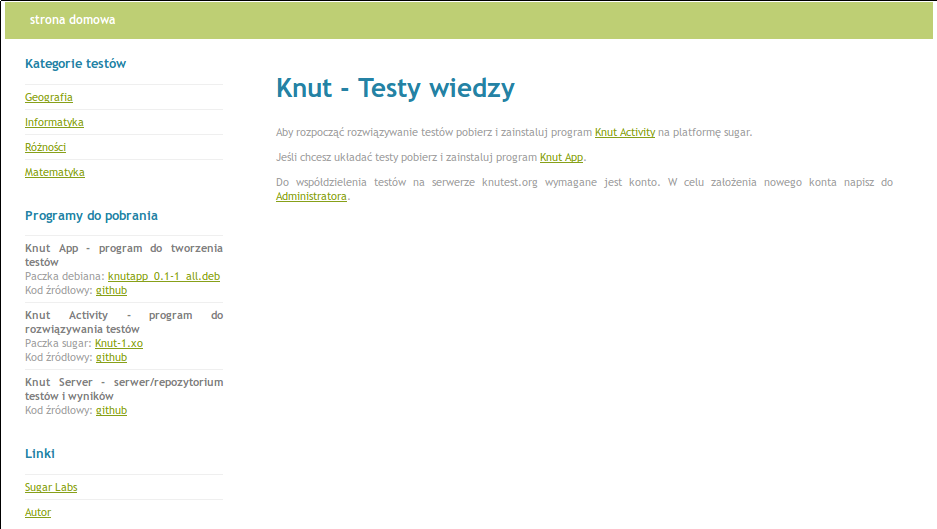
\includegraphics{StronaGlowna.png}
\end{quote}

Strona WWW prezentuje najważniejsze informacje o projekcie, pozwala na pobranie i zobaczenie kodu źródłowego programów oraz umożliwia przeglądanie opisów testów dostępnych na serwerze.


\section{Panel Administracyjny}
\label{index:id6}\label{index:panel-administracyjny}
Panel administracyjny wymaga logowania. Domyślnie logowanie odbywa się na stronie \href{http://adres\_strony/admin/}{http://adres\_strony/admin/} np. \href{http://knutest.org/admin/}{http://knutest.org/admin/}.

Logowanie do panelu administracyjnego

\scalebox{0.500000}{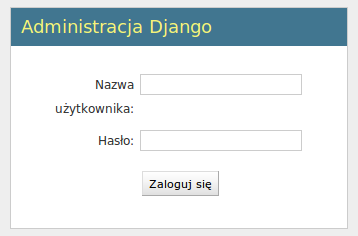
\includegraphics{Logowanie.png}}

Po podaniu prawidłowego loginu i hasła nastąpi przekierowanie do panelu administracyjnego.

Panel administracyjny

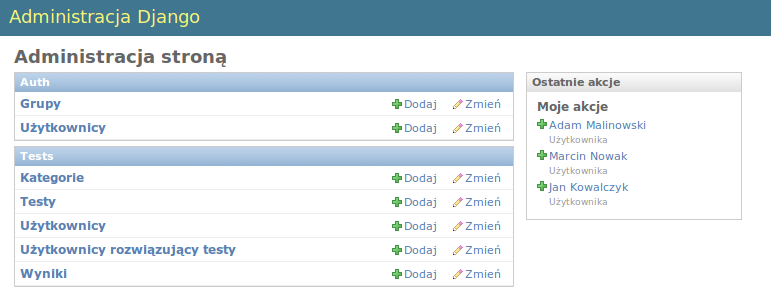
\includegraphics{Administracja.png}
\begin{description}
\item[{Panel administracyjny podzielony jest na 2 sekcje:}] \leavevmode\begin{itemize}
\item {} 
\code{Auth} - pozwala na zarządzanie administratorami serwera. Mamy możliwość definiowania grup i ich uprawnień

\item {} 
\code{Tests} - umożliwia zarządzanie testami a w szczególności zarządzanie użytkownikami edytora testów

\end{itemize}

\end{description}


\section{Zarządzanie użytkownikami edytora testów}
\label{index:zarzadzanie-uzytkownikami}\label{index:zarzadzanie-uzytkownikami-edytora-testow}
Zarządzanie użytkownikami edytora testów jest możliwe po kliknięciu na \code{Użytkownicy} w sekcji \code{Tests} panelu administracyjnego. Wyświetli się lista użytkowników.

Lista użytkowników edytora testów
\begin{quote}

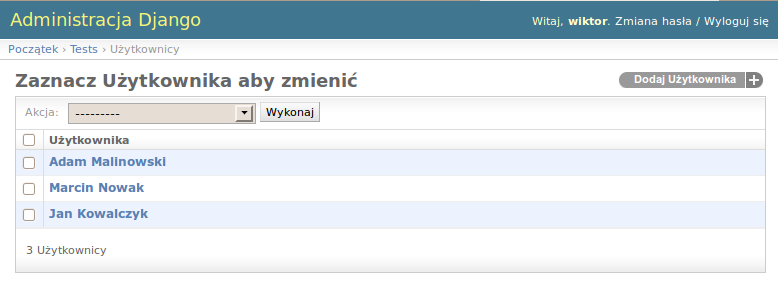
\includegraphics{ListaUzytkownikow.png}
\end{quote}

Z tej strony mamy możliwość edycji istniejących użytkowników oraz tworzenie nowych.


\subsection{Dodawanie użytkownika}
\label{index:dodawanie-uzytkownika}\begin{description}
\item[{Po kliknięciu \code{Dodaj Użytkownika} na stronie z listą użytkowników pojawi się formularz z 3 polami:}] \leavevmode\begin{itemize}
\item {} 
\code{Nazwa użytkownika} - login potrzebny do weryfikacji konta

\item {} 
\code{Hasło}

\item {} 
\code{Imię i nazwisko} - wyświetlana nazwa użytkownika

\end{itemize}

\end{description}

Dodawanie nowego użytkownika
\begin{quote}

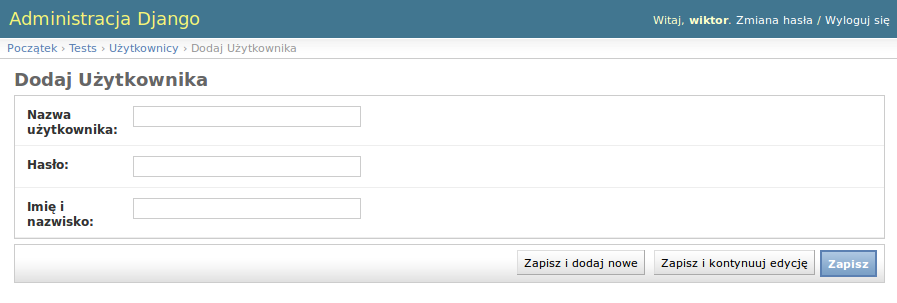
\includegraphics{DodajUzytkownika.png}
\end{quote}
\begin{description}
\item[{Po uzupełnieniu wszystkich pól należy zapisać dane. Mamy do wyboru 3 przyciski:}] \leavevmode\begin{itemize}
\item {} 
\code{Zapisz i dodaj nowe} - zapisuje wprowadzone dane i przekierowuje do nowego, pustego formularza dodawania użytkownika

\item {} 
\code{Zapisz i kontynuuj edycję} - zapisuje wprowadzone dane i zostaje na bierzącej stronie

\item {} 
\code{Zapisz} - po zapisaniu wprowadzonych danych przekierowuje do listy użytkowników edytora testów

\end{itemize}

\end{description}


\subsection{Edycja użytkownika}
\label{index:edycja-uzytkownika}
Aby edytować istniejącego użytkownika należy kliknąć na imię i nazwisko z listy użytkowników edytora testów. Pojawi się wtedy okno edycji.

Edycja użytkownika

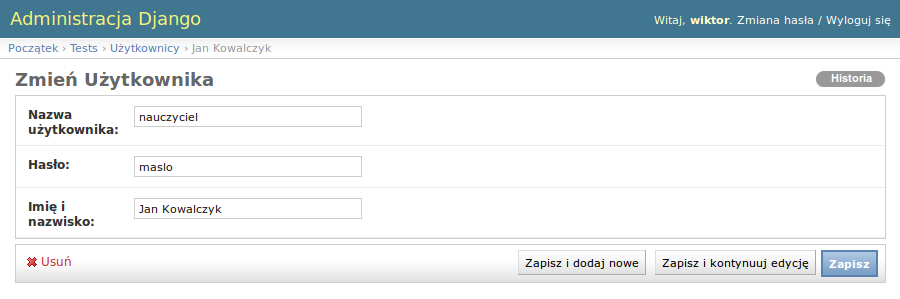
\includegraphics{EdycjaUzytkownika.png}



\renewcommand{\indexname}{Indeks}
\printindex
\end{document}
